\chapter{Analisi e discussione dei Risultati}

\section{Discussione dei Risultati}

In questa sezione vengono analizzati i risultati ottenuti attraverso l'applicazione di tre modelli di machine learning (\textit{K-Means}, \textit{Random Forest} e \textit{Convolutional Neural Network}) su cinque dataset creati per addestrare un sistema di rilevamento delle intrusioni (IDS). Ogni dataset presenta una combinazione specifica di traffico benigno e maligno, come descritto precedentemente. Il dataset per la fase di test è ottenuto selezionando una dimensione pari al 20\% dei Dataset di train dal dataset TON\_IOT, questi dati sono dati diversi da quelli utilizzati in fase di addestramento.
Le prestazioni sono misurate tramite \textit{Accuracy}, \textit{Precision}, \textit{Recall} e \textit{F1-Score}, indicatori fondamentali per valutare l'efficacia del modello nella classificazione delle intrusioni.
In particolare, per il modello Random Forest verranno valutati diversi valori di soglia, partendo dalla soglia predefinita di 0.5. Questa soglia rappresenta un punto di riferimento comune, poiché assegna una classe positiva a tutte le osservazioni per le quali la probabilità di appartenenza a quella classe supera il 50\%. Tuttavia, a seconda del contesto analizzato e degli obiettivi specifici della classificazione, è possibile esplorare ulteriori valori di soglia per ottimizzare le performance del modello. 
Ad esempio, in scenari in cui è più critico minimizzare i falsi negativi, potrebbe essere utile abbassare la soglia, consentendo a un maggior numero di osservazioni di essere classificate come positive. Viceversa, se l'obiettivo è ridurre i falsi positivi, si potrebbe alzare la soglia. 
Nei risultati che seguono quando non viene specificata una soglia alternativa, si assume automaticamente il valore di 0.5; in caso contrario, verrà esplicitamente indicata la soglia utilizzata per ogni esperimento, per garantire trasparenza e ripetibilità nei risultati ottenuti.


\subsection{Dataset 1}

\begin{figure}[htbp]
\centering
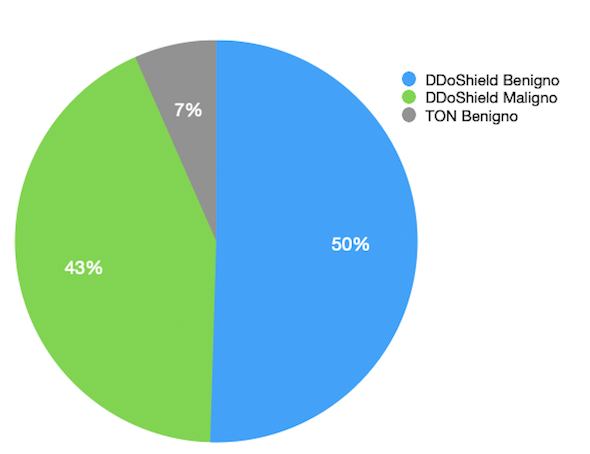
\includegraphics[scale= 0.8]{UNINA_MSc_Thesis_Project/img/chapterRisulati/composizione_DATASET_1 centrata.png}
  \caption{Composizione Dataset 1}
\end{figure}

\begin{table}[htbp]
\centering
\renewcommand{\arraystretch}{1.5} % Aumenta lo spazio tra le righe
\resizebox{\textwidth}{!}{ % Ridimensiona la tabella alla larghezza del testo
\begin{tabular}{|p{4cm}|p{3cm}|p{3cm}|p{3cm}|p{3cm}|}
\hline
\textbf{Modello} & \textbf{Accuracy \%} & \textbf{Precision \%} & \textbf{Recall \%} & \textbf{F1-Score \%} \\
\hline
\textbf{K-Means} & 84.09 & 76.54 & 98.95 & 86.31 \\
\hline
\textbf{Random Forest (RF-0.25)} & 70.74 & 100 & 42.17 & 59.32 \\
\hline
\textbf{Convolutional Neural Network (CNN)} & 66.34 & 99.66 & 33.42 & 50.06 \\
\hline
\end{tabular}
}
\caption{Metriche di performance per Dataset 1}
\label{tab:performance_metrics}
\end{table}

Il \textbf{Dataset 1} contiene traffico benigno e maligno proveniente da DDoShield, insieme al traffico benigno dal dataset TON\_IOT. I risultati ottenuti per questo dataset evidenziano una performance discreta da parte del modello \textit{K-Means}, che ha raggiunto un'accuratezza di 0.84, una precisione di 0.76, un richiamo elevato pari a 0.98 e un F1-Score di 0.86. Questo suggerisce che il modello ha una forte capacità di rilevare traffico maligno (alto richiamo), ma tende a classificare una parte del traffico benigno come maligno (Falsi Positivi), riflettendo la precisione relativamente bassa.
 
Al contrario, il \textit{CNN} ha ottenuto risultati inferiori rispetto al \textit{K-Means}, con un'accuratezza di 0.66 e un F1-Score di 0.50, indicando che il modello soffre di una bassa capacità di rilevamento del traffico maligno (richiamo di 0.33), pur mantenendo una precisione molto alta (0.99), evidenziando una tendenza a minimizzare i falsi positivi.
L'algoritmo \textit{RF} presenta prestazioni accettabili solo scegliendo una soglia minore di 0.5.
Ulteriori aspetti saranno approfonditi in seguito nel paragrafo conclusivo.

\subsection{Dataset 2}

\begin{figure}[htbp]
\centering
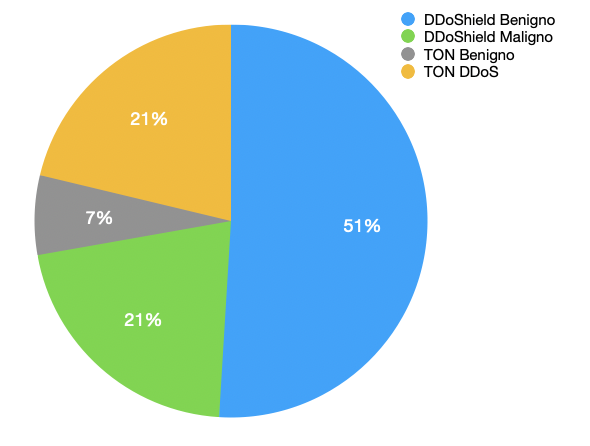
\includegraphics[scale= 0.8]{UNINA_MSc_Thesis_Project/img/chapterRisulati/composizione_DATASET_2.png}
  \caption{Composizione Dataset 2}
\end{figure}


\begin{table}[htbp]
\centering
\renewcommand{\arraystretch}{1.5} % Aumenta lo spazio tra le righe
\resizebox{\textwidth}{!}{ % Ridimensiona la tabella alla larghezza del testo
\begin{tabular}{|p{4cm}|p{3cm}|p{3cm}|p{3cm}|p{3cm}|}
\hline
\textbf{Modello} & \textbf{Accuracy \%} & \textbf{Precision \%} & \textbf{Recall \%} & \textbf{F1-Score \%} \\
\hline
\textbf{K-Means} & 86.53 & 79.60 & 98.75 & 88.14 \\
\hline
\textbf{Random Forest (RF-0.25)} & 97.40  & 95.11 & 100 & 97.49  \\
\hline
\textbf{Random Forest (RF)} & 99.95 & 99.90 & 100 & 99.95 \\
\hline
\textbf{Convolutional Neural Network (CNN)} & 99.98 & 100 & 99.97 & 99.98 \\
\hline
\end{tabular}
}
\caption{Metriche di performance per Dataset 2}
\label{tab:performance_metrics}
\end{table}

Il \textbf{Dataset 2} è stato generato combinando il traffico benigno di \textit{Dataset 1} con traffico maligno equamente distribuito tra DDoShield e TON\_IOT DDoS. Qui, \textit{K-Means} ha ottenuto risultati superiori rispetto al \textit{Dataset 1}, con un'accuratezza di 0.86 e un F1-Score di 0.88. Il miglioramento delle prestazioni si riflette anche in una precisione maggiore (0.79), che indica una riduzione dei falsi positivi.
\textit{Random Forest} ha mostrato eccellenti performance, con valori quasi perfetti (accuracy di 0.99, F1-Score di 0.99), dimostrando una notevole capacità di bilanciare la rilevazione degli attacchi tra DDoShield e TON\_IOT.
La \textit{CNN} ha ottenuto risultati simili a quelli di \textit{Random Forest}, con un'accuratezza di 0.99, mostrando come i modelli più complessi possano gestire efficacemente dataset bilanciati.

\subsection{Dataset 3}

\begin{figure}[htbp]
\centering
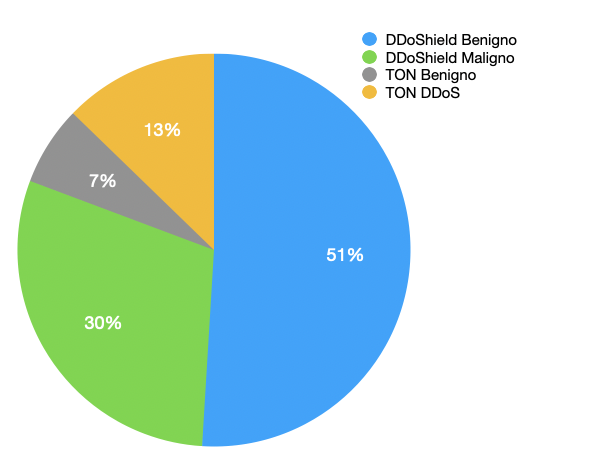
\includegraphics[scale= 0.8]{UNINA_MSc_Thesis_Project/img/chapterRisulati/composizione_DATASET_3.png}
  \caption{Composizione Dataset 3}
\end{figure}

\begin{table}[htbp]
\centering
\renewcommand{\arraystretch}{1.5} % Aumenta lo spazio tra le righe
\resizebox{\textwidth}{!}{ % Ridimensiona la tabella alla larghezza del testo
\begin{tabular}{|p{4cm}|p{3cm}|p{3cm}|p{3cm}|p{3cm}|}
\hline
\textbf{Modello} & \textbf{Accuracy \%} & \textbf{Precision \%} & \textbf{Recall \%} & \textbf{F1-Score \%} \\
\hline
\textbf{K-Means} & 86.62  & 80.71 & 96.74 & 88.00 \\
\hline
\textbf{Random Forest (RF-0.25)} & 91.18 & 1.0 & 42.17 & 95.38 \\
\hline
\textbf{Random Forest (RF)} & 100 & 100 & 100 & 100 \\
\hline
\textbf{Convolutional Neural Network (CNN)} & 67.90 & 100 & 36.41 & 53.38 \\
\hline
\end{tabular}
}
\caption{Metriche di performance per Dataset 3}
\label{tab:performance_metrics}
\end{table}

Nel \textbf{Dataset 3}, con una prevalenza di traffico maligno da DDoShield, \textit{K-Means} ha ottenuto prestazioni comparabili al \textit{Dataset 2}, con un'accuratezza di 0.86 e un F1-Score di 0.88, mantenendo un buon bilanciamento tra precisione e richiamo.
\textit{Random Forest} ha nuovamente raggiunto risultati perfetti, dimostrando la sua capacità di gestire dataset sbilanciati. Tuttavia, la \textit{CNN} ha sofferto un calo significativo (accuratezza di 0.67 e F1-Score di 0.53), indicando che l'architettura neurale potrebbe avere difficoltà nel rilevare intrusioni in dataset con distribuzioni sbilanciate tra diverse tipologie di traffico maligno.

\subsection{Dataset 4}

\begin{figure}[htbp]
\centering
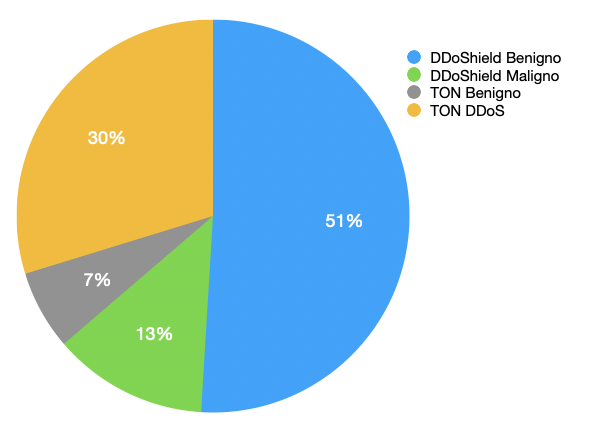
\includegraphics[scale= 0.8]{UNINA_MSc_Thesis_Project/img/chapterRisulati/composizione_DATASET_4.png}
  \caption{Composizione Dataset 4}
\end{figure}

\begin{table}[htbp]
\centering
\renewcommand{\arraystretch}{1.5} % Aumenta lo spazio tra le righe
\resizebox{\textwidth}{!}{ % Ridimensiona la tabella alla larghezza del testo
\begin{tabular}{|p{4cm}|p{3cm}|p{3cm}|p{3cm}|p{3cm}|}
\hline
\textbf{Modello} & \textbf{Accuracy \%} & \textbf{Precision \%} & \textbf{Recall \%} & \textbf{F1-Score \%} \\
\hline
\textbf{K-Means} & 84.07  & 78.26 & 94.97 & 85.81 \\
\hline
\textbf{Random Forest (RF-0.25)} & 93.30 & 88.28 & 100 & 93.78 \\
\hline
\textbf{Random Forest (RF)} & 99.91 & 99.83 & 100 & 99.91 \\
\hline
\textbf{Convolutional Neural Network (CNN)} & 99.60 & 100 & 99.22 & 99.60 \\
\hline
\end{tabular}
}
\caption{Metriche di performance per Dataset 4}
\label{tab:performance_metrics}
\end{table}

Nel \textbf{Dataset 4}, caratterizzato da una maggioranza di traffico maligno da TON\_IOT DDoS, \textit{K-Means} ha mostrato una leggera diminuzione delle performance (accuratezza di 0.84, F1-Score di 0.85), a causa di un aumento dei falsi positivi, come indicato dalla precisione di 0.78.
\textit{Random Forest} continua a mantenere prestazioni eccellenti, con un'accuratezza di 0.9991 e metriche molto elevate, mentre la \textit{CNN}, con un'accuratezza di 0.99, ha dimostrato di gestire meglio dataset con una predominanza di traffico maligno da TON\_IOT rispetto a quanto visto nel \textit{Dataset 3}.

\subsection{Dataset 5}

\begin{figure}[htbp]
\centering
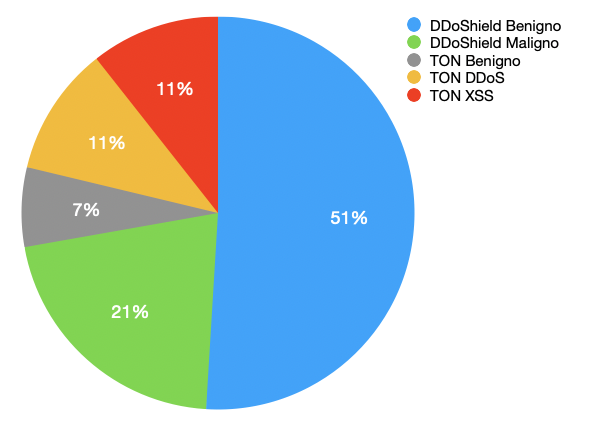
\includegraphics[scale= 0.8]{UNINA_MSc_Thesis_Project/img/chapterRisulati/composizione_DATASET_5.png}
  \caption{Composizione Dataset 5}
\end{figure}

\begin{table}[htbp]
\centering
\renewcommand{\arraystretch}{1.5} % Aumenta lo spazio tra le righe
\resizebox{\textwidth}{!}{ % Ridimensiona la tabella alla larghezza del testo
\begin{tabular}{|p{4cm}|p{3cm}|p{3cm}|p{3cm}|p{3cm}|}
\hline
\textbf{Modello} & \textbf{Accuracy \%} & \textbf{Precision \%} & \textbf{Recall \%} & \textbf{F1-Score \%} \\
\hline
\textbf{K-Means} & 86.31  & 86.42 & 94.48 & 90.27 \\
\hline
\textbf{Random Forest (RF-0.25)} & 76.48 & 74.04 & 100 & 85.08 \\
\hline
\textbf{Random Forest (RF)} & 99.99 & 99.99 & 100 & 99.99 \\
\hline
\textbf{Convolutional Neural Network (CNN)} & 96.96 & 99.96 & 95.50 & 97.68 \\
\hline
\end{tabular}
}
\caption{Metriche di performance per Dataset 5}
\label{tab:performance_metrics}
\end{table}

Il \textbf{Dataset 5} introduce traffico XSS nel dataset, rendendo la classificazione più complessa. Nonostante ciò, \textit{K-Means} ha mantenuto buone prestazioni con un'accuratezza di 0.8631 e un F1-Score di 0.90. La precisione è aumentata (0.86), suggerendo che il modello ha migliorato la sua capacità di evitare falsi positivi in presenza di una maggiore varietà di traffico maligno.

\textit{Random Forest} ha nuovamente raggiunto valori quasi perfetti (accuratezza di 0.99), dimostrando la sua capacità di rilevare diverse tipologie di attacchi con alta precisione. La \textit{CNN} ha mostrato una buona capacità di generalizzazione, con un'accuratezza di 0.96 e un F1-Score di 0.97, dimostrando che riesce a gestire anche dataset più complessi con traffico misto (DDoS e XSS).

\subsection{Analisi dei Risultati}
In questa sezione analizziamo i risultati ottenuti dai vari algoritmi applicati sui differenti dataset descritti in precedenza. Ogni algoritmo ha mostrato prestazioni diverse a seconda delle caratteristiche del dataset, il che ci permette di identificare alcune peculiarità nei loro comportamenti.

\subsubsection{K-Means}
\textit{K-Means} è un algoritmo di clustering non supervisionato che raggruppa i dati basandosi sulla similarità, utilizzando la distanza euclidea per creare cluster. Sebbene non sia nato come algoritmo di classificazione, può essere adattato per tale scopo. Tuttavia, ha dimostrato prestazioni variabili a seconda del dataset considerato.
Nel \textbf{Dataset 1} e nel \textbf{Dataset 2}, dove la separazione tra classi è relativamente chiara, \textit{K-Means} ha ottenuto ottimi risultati, con accuratezze superiori all'84\%. Questo suggerisce che l'algoritmo riesce a sfruttare efficacemente la differenza strutturale tra traffico benigno e maligno quando questa è ben definita.
Con dataset più complessi, come il \textbf{Dataset 3} e il \textbf{Dataset 4}, in cui c'è uno squilibrio tra le classi, \textit{K-Means} ha mostrato un leggero calo delle performance. Sebbene la precisione sia rimasta alta (indicando che il modello fa poche previsioni errate quando etichetta un pacchetto come maligno), l'accuratezza complessiva e il richiamo sono diminuiti leggermente. Questo è indicativo del fatto che \textit{K-Means} fatica a distinguere intrusioni meno evidenti, suggerendo che l'algoritmo è eccessivamente conservativo nel segnalare traffico maligno, risultando in un elevato numero di falsi negativi.

\subsubsection{Random Forest (RF)}
\textit{Random Forest} è un algoritmo di classificazione supervisato che utilizza un insieme di alberi decisionali per creare un modello robusto. Grazie alla sua capacità di catturare interazioni complesse tra le variabili, RF ha ottenuto eccellenti prestazioni su quasi tutti i dataset, mantenendo accuratezze vicine al 100\%.
In particolare, \textit{Random Forest} ha gestito in modo eccellente i dataset più complessi come il \textbf{Dataset 3} e il \textbf{Dataset 5}, dove il traffico maligno proveniva da fonti diverse (DDoS e XSS) e presentava una variabilità maggiore. Le alte prestazioni di RF sono dovute alla capacità dell'algoritmo di gestire la variabilità dei dati e catturare pattern non lineari, riducendo così il rischio di falsi negativi o positivi. Questo conferma l'idoneità di \textit{Random Forest} nel contesto della rilevazione delle intrusioni, anche in scenari con distribuzioni di dati complesse e sbilanciate.

\subsubsection{Convolutional Neural Network (CNN)}
Le \textit{Convolutional Neural Networks} sono reti neurali particolarmente adatte all'analisi di dati con struttura gerarchica, come immagini o dati con pattern temporali. Tuttavia, le prestazioni della \textit{CNN} sono state variabili a seconda del dataset utilizzato.
Nel \textbf{Dataset 1} e \textbf{Dataset 3}, la CNN ha mostrato prestazioni inferiori rispetto agli altri algoritmi, con un'accuratezza di circa il 66\% e il 68\%, rispettivamente. Questo può essere attribuito al fatto che questi dataset non fornivano sufficiente complessità o variazione nei dati per permettere alla CNN di esprimere appieno le sue capacità. In particolare, nel \textbf{Dataset 3}, la precisione è risultata molto alta (1.0), ma il richiamo è stato estremamente basso (0.36), indicando che la CNN era estremamente selettiva nel classificare un pacchetto come maligno, trascurando però molti pacchetti malevoli (alto numero di falsi negativi).
D'altro canto, nel \textbf{Dataset 5}, che conteneva traffico DDoS e XSS, la CNN ha mostrato le sue migliori prestazioni, con un'accuratezza del 96.96\%. In questo caso, la complessità dei dati ha permesso alla CNN di identificare più efficacemente pattern distintivi tra le diverse tipologie di attacchi.

\subsubsection{Sintesi dell'analisi}
L'analisi dei risultati mostra che le differenze nelle prestazioni degli algoritmi dipendono principalmente dalla complessità del dataset e dalla distribuzione delle classi:
\begin{itemize}
\item \textbf{K-Means} funziona bene su dataset bilanciati e con classi chiaramente separate, come \textit{Dataset 1} e \textit{Dataset 2}. Tuttavia, fatica in presenza di classi meno ben distinte o dataset più complessi con un numero di falsi positivi che potrebbe aumentare.
\item \textbf{Random Forest} si dimostra un algoritmo flessibile e robusto, con prestazioni costantemente elevate su tutti i dataset, grazie alla sua capacità di gestire interazioni complesse e dati sbilanciati.
\item \textbf{CNN} mostra prestazioni variabili, eccellendo solo nei dataset più complessi (\textit{Dataset 5}), dove è in grado di identificare pattern intricati. Tuttavia, ha evidenziato difficoltà con dataset fortemente sbilanciati come il \textit{Dataset 3} e con pochi dati a supporto, suggerendo che potrebbe necessitare di ulteriori ottimizzazioni per gestire questi scenari.
\end{itemize}
In particolare, è importante sottolineare che \textit{Random Forest} è un algoritmo capace di cogliere relazioni non lineari, il che si riflette in un comportamento più bilanciato anche in presenza di dataset eterogenei. Le reti neurali, sebbene siano in grado di rilevare pattern complessi cosi come \textit{Random Forest}, soffrono maggiormente \textbf{la dipendenza dai dati} e richiedono una mole maggiore di dati per un addestramento efficace. Questo spiega i risultati inferiori ottenuti sui \textit{Dataset 1} e \textit{Dataset 3}, che sono fortemente sbilanciati a favore del simulatore.
Concludendo, \textbf{Random Forest} emerge come la scelta più solida per la rilevazione delle intrusioni nei dataset utilizzati, mentre \textit{CNN} e \textit{K-Means} mostrano prestazioni buone solo in contesti specifici, a seconda della struttura dei dati.

\section{L'impatto della strategia}

Per valutare l'impatto della tecnica di addestramento e del lavoro svolto, in questa sezione analizziamo gli stessi dataset senza l'uso del simulatore \textit{DDoShield}. L'obiettivo è simulare scenari nei quali non avremmo avuto il supporto del simulatore, consentendo di valutare il contributo effettivo di \textit{DDoShield} in condizioni reali. Il confronto delle performance con e senza il simulatore è fondamentale per dimostrare l'importanza del tool, soprattutto in presenza di dataset fortemente sbilanciati. In questi casi, infatti, vedremo come i dati, senza il simulatore, risulterebbero difficilmente utilizzabili.

Le metriche nelle tabelle seguenti saranno presentate nel seguente formato:
\[metrica\_DATASET\_TON\_Only_i [metrica\_DATASET_i]\]
dove \[DATASET_i\] con i=1,2,3,4,5 rappresenta gli scenari precedentemente generati.



\subsection{Dataset2 TON\_Only}

\begin{figure}[htbp]
\centering
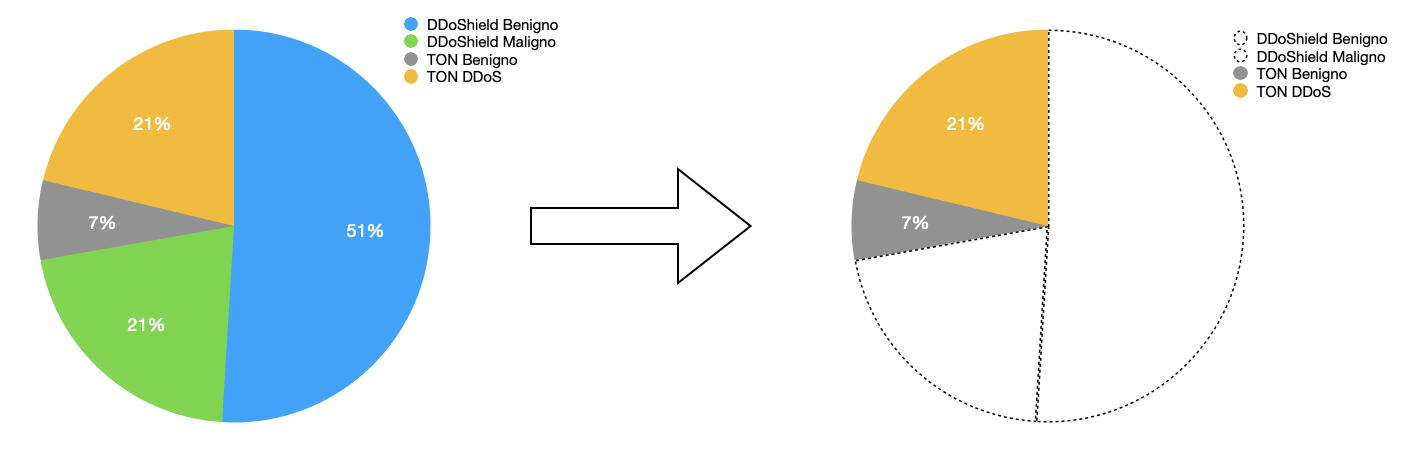
\includegraphics[scale= 0.6]{UNINA_MSc_Thesis_Project/img/chapterRisulati/TON_Only/composizione_TON_ONLY2.png}
  \caption{Composizione Dataset TON Only 2}
\end{figure}

\begin{table}[htbp]
\centering
\renewcommand{\arraystretch}{1.5}
\resizebox{\textwidth}{!}{
\begin{tabular}{|p{4cm}|p{3cm}|p{3cm}|p{3cm}|p{3cm}|}
\hline
\textbf{Modello} & \textbf{Accuracy \%} & \textbf{Precision \%} & \textbf{Recall \%} & \textbf{F1-Score \%} \\
\hline
\textbf{K-Means} & 98.47 [86.53] & 97.49 [79.60] & 99.57 [98.75] & 98.52 [88.14] \\
\hline
\textbf{Random Forest (RF-0.25)} & 49.34 [97.40] & 100 [95.11] & 0.02 [100] & 0.05 [97.49] \\
\hline
\textbf{Random Forest (RF-0.5)} & 49.34 [99.95] & 0 [99.90] & 0 [100] & 0 [99.95] \\
\hline
\textbf{Convolutional Neural Network (CNN)} & 93.16 [99.98] & 99.68 [100] & 86.77 [99.97] & 92.78 [99.98] \\
\hline
\end{tabular}
}
\caption{Metriche di performance per Dataset2 TON\_Only}
\label{tab:performance_metrics}
\end{table}
Nel Dataset2, l'uso del simulatore ha un impatto positivo su tutti i modelli, tranne che su \textit{K-Means}, dove la differenza è meno pronunciata. In particolare, il \textit{Random Forest} senza simulatore mostra risultati estremamente scarsi, con un \textit{recall} praticamente nullo, mentre con il simulatore il modello raggiunge performance ottimali in tutte le metriche. La \textit{CNN} mostra un comportamento simile, con un significativo miglioramento nell'accuratezza, precisione e \textit{recall} grazie al simulatore.

\subsection{Dataset3 TON\_Only}

\begin{figure}[htbp]
\centering
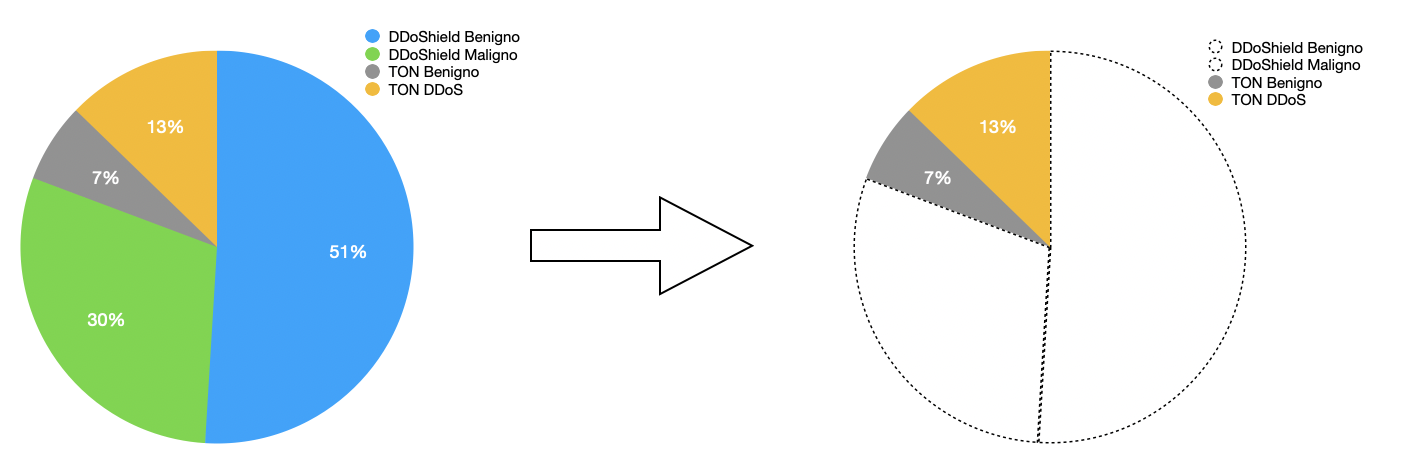
\includegraphics[scale= 0.6]{UNINA_MSc_Thesis_Project/img/chapterRisulati/TON_Only/composizione_TON_ONLY3.png}
  \caption{Composizione Dataset TON Only 3}
\end{figure}


\begin{table}[htbp]
\centering
\renewcommand{\arraystretch}{1.5}
\resizebox{\textwidth}{!}{
\begin{tabular}{|p{4cm}|p{3cm}|p{3cm}|p{3cm}|p{3cm}|}
\hline
\textbf{Modello} & \textbf{Accuracy \%} & \textbf{Precision \%} & \textbf{Recall \%} & \textbf{F1-Score \%} \\
\hline
\textbf{K-Means} & 97.40 [86.62] & 95.15 [80.71] & 100 [96.74] & 97.51 [88.00] \\
\hline
\textbf{Random Forest (RF-0.25)} & 57.72 [95.11] & 54.51 [91.18] & 100 [100] & 70.56 [95.38] \\
\hline
\textbf{Random Forest (RF-0.5)} & 86.44 [100] & 78.12 [100] & 100 [100] & 88.29 [100] \\
\hline
\textbf{Convolutional Neural Network (CNN)} & 98.89 [67.90] & 97.87 [100] & 100 [36.41] & 98.92 [53.38] \\
\hline
\end{tabular}
}
\caption{Metriche di performance per Dataset3 TON\_Only}
\label{tab:performance_metrics}
\end{table}
Nel Dataset3, il simulatore migliora significativamente le prestazioni del \textit{Random Forest}. Nel \textit{K-Means}, i risultati senza simulatore sono più elevati. La \textit{CNN} mostra un comportamento interessante: mentre la precisione rimane alta, il \textit{recall} e quindi anche l'F1-score peggiorano drasticamente senza simulatore, ricordiamo che questo dataset risultava pesantemente sbilanciato ai dati del simulatore. 

\subsection{Dataset4 TON\_Only}

\begin{figure}[htbp]
\centering
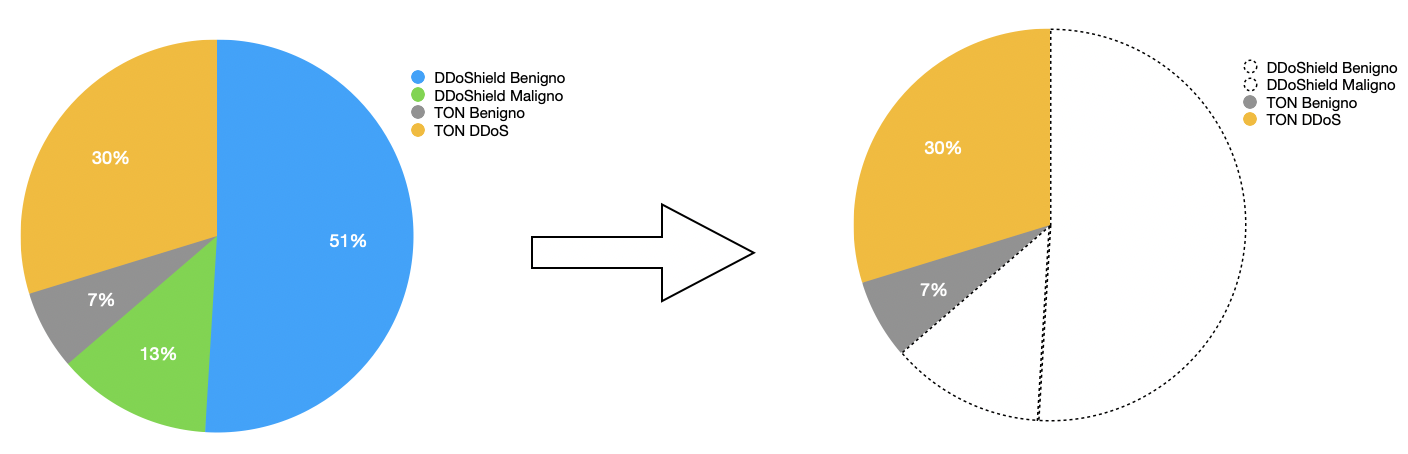
\includegraphics[scale= 0.6]{UNINA_MSc_Thesis_Project/img/chapterRisulati/TON_Only/composizione_TON_ONLY4.png}
  \caption{Composizione Dataset TON Only 4}
\end{figure}

\begin{table}[htbp]
\centering
\renewcommand{\arraystretch}{1.5}
\resizebox{\textwidth}{!}{
\begin{tabular}{|p{4cm}|p{3cm}|p{3cm}|p{3cm}|p{3cm}|}
\hline
\textbf{Modello} & \textbf{Accuracy \%} & \textbf{Precision \%} & \textbf{Recall \%} & \textbf{F1-Score \%} \\
\hline
\textbf{K-Means} & 97.03 [84.07] & 94.50 [78.26] & 100 [94.97] & 97.17 [85.81] \\
\hline
\textbf{Random Forest (RF-0.25)} & 57.18 [93.30] & 54.14 [88.28] & 100 [100] & 70.00 [93.78] \\
\hline
\textbf{Random Forest (RF-0.5)} & 86.21 [99.91] & 78.46 [99.83] & 100 [100] & 88.46 [99.91] \\
\hline
\textbf{Convolutional Neural Network (CNN)} & 98.82 [99.60] & 97.72 [100] & 100 [99.22] & 98.85 [99.60] \\
\hline
\end{tabular}
}
\caption{Metriche di performance per Dataset4 TON\_Only}
\label{tab:performance_metrics}
\end{table}

Per il Dataset4, si osserva un miglioramento generale delle performance con l'uso del simulatore, specialmente per \textit{Random Forest} e \textit{CNN}, mentre il \textit{K-Means} risulta più stabile anche senza simulatore. Questo indica che il simulatore aiuta i modelli più complessi a gestire meglio dataset con distribuzioni più eterogenee e difficili da prevedere.

\subsection{Dataset5 TON\_Only}

\begin{figure}[htbp]
\centering
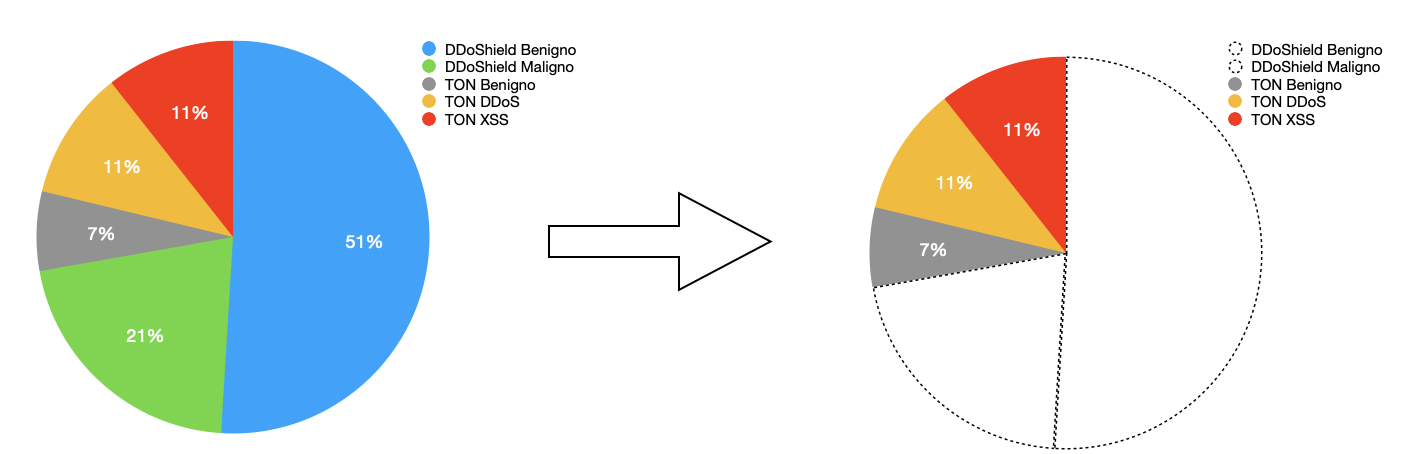
\includegraphics[scale= 0.6]{UNINA_MSc_Thesis_Project/img/chapterRisulati/TON_Only/composizione_TON_ONLY5.png}
  \caption{Composizione Dataset TON Only 5}
\end{figure}

\begin{table}[htbp]
\centering
\renewcommand{\arraystretch}{1.5}
\resizebox{\textwidth}{!}{
\begin{tabular}{|p{4cm}|p{3cm}|p{3cm}|p{3cm}|p{3cm}|}
\hline
\textbf{Modello} & \textbf{Accuracy \%} & \textbf{Precision \%} & \textbf{Recall \%} & \textbf{F1-Score \%} \\
\hline
\textbf{K-Means} & 97.85 [86.31] & 96.03 [86.42] & 99.92 [94.48] & 97.94 [90.27] \\
\hline
\textbf{Random Forest (RF-0.25)} & 52.28 [76.48] & 51.50 [74.04] & 100 [100] & 67.99 [85.08] \\
\hline
\textbf{Random Forest (RF-0.5)} & 99.90 [99.99] & 99.92 [99.99] & 100 [100] & 99.91 [99.99] \\
\hline
\textbf{Convolutional Neural Network (CNN)} & 98.50 [96.96] & 98.25 [99.96] & 99.85 [95.50]
 & 98.92 [97.68] \\
\hline
\end{tabular}
}
\caption{Metriche di performance per Dataset5 TON\_Only}
\label{tab:performance_metrics}
\end{table}

Anche nel Dataset5, l'uso del simulatore porta a miglioramenti significativi per tutti i modelli, ad eccezione del \textit{K-Means} che mostra performance più elevate senza il simulatore. Questo comportamento potrebbe essere dovuto alla capacità del \textit{K-Means} di lavorare meglio con i dati "naturali" e meno strutturati.

\subsection{Conclusioni Generali sui Risultati}

Dai risultati ottenuti attraverso i vari dataset, possiamo trarre diverse conclusioni riguardo l'efficacia del simulatore \textit{DDoShield} e il suo impatto sulle prestazioni dei modelli testati.
In generale, l'utilizzo del simulatore ha migliorato significativamente le prestazioni di modelli complessi come \textit{Random Forest} e \textit{Convolutional Neural Network (CNN)}. Questo miglioramento è particolarmente evidente in dataset sbilanciati, dove il simulatore ha fornito un contributo fondamentale per bilanciare le classi e consentire al modello di apprendere meglio anche in presenza di attacchi più rari o complessi. Le metriche di \textit{accuracy}, \textit{precision}, \textit{recall} e \textit{F1-score} mostrano chiaramente che, senza il simulatore, i modelli soffrono di un significativo calo di performance, specialmente in termini di \textit{recall} e \textit{F1-score}, suggerendo difficoltà nel riconoscere correttamente le classi di attacco.
D'altra parte, il modello \textit{K-Means} ha mostrato un comportamento meno dipendente dal simulatore, con risultati sempre migliori senza l'uso di dati simulati.

\textbf{Random Forest}: Il \textit{Random Forest} ha tratto il massimo beneficio dal simulatore, passando da performance pessime in assenza del simulatore a performance ottimali quando i dati simulati erano inclusi. Ciò indica che il modello è altamente sensibile al bilanciamento delle classi e alla varietà dei dati, che il simulatore è stato in grado di fornire. Senza il simulatore, infatti, in alcuni casi il modello non riusciva nemmeno a identificare correttamente le classi di attacco, con un \textit{recall} e un \textit{F1-score} prossimi allo zero.

\textbf{Convolutional Neural Network (CNN)}: Anche il modello \textit{CNN} ha beneficiato significativamente dell'uso del simulatore, mostrando un miglioramento in quasi tutte le metriche. Tuttavia, sono emersi anche casi in cui il modello ha presentato un calo di performance nel \textit{recall}, specialmente per dataset molto sbilanciati. Questo suggerisce che, sebbene il simulatore abbia migliorato la capacità della \textit{CNN} di apprendere dai dati, rimane una certa vulnerabilità del modello nel gestire alcune classi di attacco più complesse e povere di dati.

\textbf{K-Means}: L'algoritmo \textit{K-Means} presenta un caso particolare, poiché per tutti i dataset testati le performance sono risultate superiori senza l'uso dei dati simulati. Questo suggerisce che i cluster naturali nel dataset non simulato sono più facilmente identificabili da algoritmi di clustering non supervisionato rispetto ai dati generati. Questa condizione porta a performance molto elevate anche in presenza di un numero ridotto di dati, come nel \textit{Dataset 4}. In questo caso, l'introduzione del simulatore genera un aumento del rumore, comportando una difficoltà nelle predizioni.

\subsection{Conclusioni}
Complessivamente, i risultati indicano che il simulatore \textit{DDoShield} ha un impatto estremamente positivo sui modelli di apprendimento supervisionato, come \textit{Random Forest} e \textit{CNN}, migliorando significativamente la capacità di questi modelli di gestire dataset sbilanciati e di riconoscere correttamente le classi di attacco. Inoltre, il simulatore risulta comunque utile anche con \textit{K-Means}, per evitare problemi di overfitting.
Pertanto, possiamo concludere che l'uso di un simulatore come \textit{DDoShield} è fortemente raccomandato in scenari di classificazione e riconoscimento di attacchi, in particolare quando si impiegano modelli di apprendimento supervisionato e si lavora con dataset sbilanciati. 

%Tuttavia, nel caso di algoritmi come le CNN, è fondamentale prestare attenzione a non introdurre una quantità eccessiva di dati simulati, poiché ciò potrebbe ri-sbilanciare il dataset. Gli esperimenti condotti suggeriscono di mantenere la proporzione di dati simulati al di sotto del 70\% per garantire risultati ottimali.


\section{Repository GitHub}

Tutto il codice sviluppato e i dataset utilizzati per questa tesi sono disponibili pubblicamente su GitHub. Questa repository è stato creata con l'obiettivo di garantire la riproducibilità del lavoro svolto, consentendo ad altri ricercatori e professionisti di replicare gli esperimenti e, eventualmente, migliorare le metodologie proposte. 

La repository GitHub include i seguenti elementi:
\begin{itemize}
    \item Il codice sorgente per la generazione dei dataset utilizzati nei diversi esperimenti.
    \item Gli script utilizzati per l'addestramento dei modelli di machine learning, inclusi ulteriori algoritmi oltre quelli proposti in questo lavoro.
    %\item I risultati ottenuti, presentati in forma di report e grafici che riassumono le metriche di valutazione per ogni modello.
    \item La documentazione tecnica relativa al setup dell'ambiente di simulazione e alla creazione dei dataset a partire dai pacchetti catturati durante il traffico di rete.
\end{itemize}
Per accedere alla repository, è possibile visitare il seguente link:

\begin{quote}
\href{https://github.com/Luigi-Cerrato/ThesisRepository}{https://github.com/Luigi-Cerrato/ThesisRepository}
\end{quote}
La pubblicazione su GitHub non solo rende i dati e il codice liberamente accessibili, ma promuove anche un approccio collaborativo e aperto alla ricerca. Chiunque può contribuire con suggerimenti, correzioni o ulteriori sviluppi attraverso il sistema di pull request e issue tracking messo a disposizione dalla piattaforma.
In un contesto di ricerca sempre più orientato verso l'open science, questa scelta riflette l'importanza di condividere conoscenze e strumenti per accelerare i progressi nel campo della sicurezza informatica e dell'addestramento di Intrusion Detection Systems (IDS).
